\documentclass{math}

\usepackage{tikz}
\usetikzlibrary{arrows.meta}

\title{Differential Equations}
\author{Alvin Lin}
\date{January 2018 - May 2018}

\begin{document}

\maketitle

\section*{Laplace Transforms}
Let \( f \) be a function defined on \( [0,\infty) \). The Laplace transform
of \( f \), \( \laplace{f(s)} \), is a function \( F(s) \), where \( s \)
is the new variable. The domain of \( \laplace{f} \), or \( F(s) \), is all
values of \( s \) for which the following converges:
\[ \laplace{f} = \int_{0}^{\infty}\e^{-st}f(t)\diff{t} \]
Recall the following:
\[ \int_{0}^{\infty}g(t)\diff{t} = \lim_{N\to\infty}\int_{0}^{N}g(t)\diff{t} \]
If this limit exists, it converges. Otherwise, it diverges.

\subsubsection*{Example}
Find \( \laplace{f(t)} \) where \( f(t) = 1 \).
\begin{align*}
  \laplace{1} &= \int_{0}^{\infty}\e^{-st}\diff{t} \\
  &= \lim_{N\to\infty}\int_{0}^{\infty}\e^{-st}\diff{t} \\
  &= \lim_{N\to\infty}\bigg[-\frac{1}{s}\e^{-st}\bigg]_{0}^{N} \\
  &= \lim_{N\to\infty}\bigg[-\frac{1}{\e^{sN}}-\bigg(-\frac{1}{s}\bigg)\bigg] \\
  &= \frac{1}{s}, \quad s > 0
\end{align*}
Additional fact: \( \laplace{0} = 0 \).

\subsubsection*{Example}
Find \( \laplace{\e^{at}} \) where \( a \) is real.
\begin{align*}
  f(t) &= \e^{at} \\
  \laplace{\e^{at}} &= \int_{0}^{\infty}\e^{-st}\e^{at}\diff{t} \\
  &= \int_{0}^{\infty}\e^{-(s-a)t}\diff{t} \\
  &= \lim_{N\to\infty}\int_{0}^{N}\e^{-(s-a)t}\diff{t} \\
  &= \lim_{N\to\infty}\bigg[-\frac{1}{s-a}\e^{-(s-a)t}\bigg]_{0}^{N} \\
  &= \lim_{N\to\infty}\bigg[-\frac{1}{s-a}\e^{-(s-a)N}-
    \bigg(-\frac{1}{s-a}\bigg)\bigg] \\
  &= \lim_{N\to\infty}-\frac{1}{s-a}\e^{-(s-a)N}+\frac{1}{s-a} \\
  &= \frac{1}{s-a}, \quad s-a > 0 \\
  &= \frac{1}{s-a}, \quad s>a \\
  \laplace{\e^{2t}} &= \frac{1}{s-2} \\
  \laplace{\e^{-2t}} &= \frac{1}{s+2}
\end{align*}

\subsubsection*{Example}
Find \( \laplace{t} \).
\begin{align*}
  f(t) &= t \\
  \laplace{t} &= \int_{0}^{\infty}t\e^{-st}\diff{t} \\
  &= \lim_{N\to\infty}\int_{0}^{N}t\e^{-st}\diff{t} \\
\end{align*}
\begin{align*}
  &= \lim_{N\to\infty}\bigg[-\frac{1}{s}\e^{-st}t\bigg]_{0}^{N}-
    \int_{0}^{N}-\frac{1}{s}\e^{-st}\diff{t} \\
  &= \lim_{N\to\infty}\bigg[
    -\frac{1}{s}\e^{-st}t+\frac{1}{s}(-\frac{1}{s}\e^{-st})\bigg]_{0}^{N}
  &= \lim_{N\to\infty}\bigg[
    (-\frac{1}{s}\e^{-sN}N)+(-\frac{1}{s^2}\e^{-sN}-\frac{1}{s^2})\bigg] \\
  &= \frac{1}{s^2}, \quad s>0
\end{align*}
As a general rule, for \( f(t) = t^n \) where \( n \) is a non-negative integer:
\begin{align*}
  \laplace{t^n} &= \frac{n!}{s^{n+1}} \\
  \laplace{t^3} &= \frac{3!}{s^{3+1}} = \frac{6}{s^4}
\end{align*}
Additionally, for sines and cosines:
\begin{align*}
  \laplace{\sin(bt)} &= \frac{b}{s^2+b^2}, \quad s>0,b\ne0 \\
  \laplace{\cos(bt)} &= \frac{s}{s^2+b^2}, \quad s>0,b\ne0 \\
  \laplace{\sin(\sqrt{2}t)} &= \frac{\sqrt{2}}{s^2+2} \\
  \laplace{\cos(\sqrt{2}t)} &= \frac{s}{s^2+2}
\end{align*}

\subsection*{Property of Linearity}
Given \( f(t),g(t) \) and \( k \) a constant:
\begin{enumerate}
  \item \( \laplace{f(t)\pm g(t)} = \laplace{f(t)}\pm\laplace{g(t)} \)
  \item \( \laplace{kf(t)} = k\laplace{f(t)} \)
\end{enumerate}

\subsubsection*{Example}
\[ \laplace{7+5\e^{-7t}-7\sin(3t)+7t^2+5\cos(7t)} \]
\begin{align*}
  &= \laplace{7}+\laplace{5\e^{-7t}}-\laplace{7\sin(3t)}+\laplace{7t^2}+
    \laplace{5\cos(7t)} \\
  &= 7\laplace{1}+5\laplace{\e^{-7t}}-7\laplace{\sin(3t)}+7\laplace{t^2}+
    5\laplace{\cos(7t)} \\
  &= \frac{7}{s}+\frac{5}{s+7}-\frac{(7)(3)}{s^2+9}+\frac{(7)(2!)}{s^3}+
    \frac{5s}{s^2+49}, \quad s>0
\end{align*}
Note that each term has a different condition for \( s \), so we need to take
the intersection of the conditions.

\subsection*{Existence of the Transform}
Consider a piecewise continuous function \( f \) over \( [a,b] \). \( f \) has
a finite number of jump discontinuities.
\begin{center}
  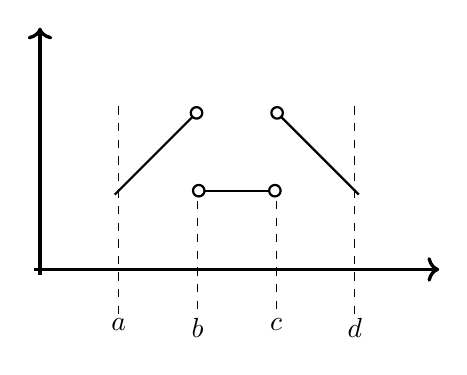
\begin{tikzpicture}[shorten >=-2pt,shorten <=-2pt]
    \draw[->,very thick] (0,0) -- (5,0);
    \draw[->,very thick] (0,0) -- (0,3);
    \draw[dashed] (1,2) -- (1,-0.5) node[below] {\( a \)};
    \draw[thick,-{Circle[open]}] (1,1) -- (2,2);
    \draw[dashed] (2,0.8) -- (2,-0.5) node[below] {\( b \)};
    \draw[thick,{Circle[open]}-{Circle[open]}] (2,1) -- (3,1);
    \draw[dashed] (3,0.8) -- (3,-0.5) node[below] {\( c \)};
    \draw[thick,{Circle[open]}-] (3,2) -- (4,1);
    \draw[dashed] (4,2) -- (4,-0.5) node[below] {\( d \)};
  \end{tikzpicture}
\end{center}
We can extend over \( [0,\infty) \). A function \( f \) is piecewise continuous
over \( [0,\infty) \) if \( f \) is piecewise continuous over \( [0,N] \) for
all \( N > 0 \).
\[ \int_{a}^{d}f(t) = \int_{a}^{b}f(t)+\int_{b}^{c}f(t)+\int_{c}^{d}f(t) \]

\subsection*{Exponential Order \( \alpha \)}
A function \( f \) is of exponential order \( \alpha \) if there exists
positive constants \( M \) and \( T \) such that \( |f(t)|\le M\e^{\alpha t} \)
for all \( t > T \).

\subsubsection*{Example}
\begin{align*}
  f(t) &= \e^{2t}\sin(t) \\
  |\e^{2t}\sin(t)| &= \e^{2t}|\sin(2t)| \le
    M\e^{2t} = \e^{2t} \text{ for all } T \\
  |\sin(2t)| &\le 1
\end{align*}
\( f(t) \) is of exponential order \( \alpha = 2 \).

\subsection*{Theorem}
Conditions for existence of the Laplace transform:
\begin{enumerate}
  \item If \( f(t) \) is piecewise continuous and of exponential order
  \( \alpha \), then the Laplace transform \( \laplace{f(t)} \) exists for
  \( s>a \).
\end{enumerate}

\begin{center}
  You can find all my notes at \url{http://omgimanerd.tech/notes}. If you have
  any questions, comments, or concerns, please contact me at
  alvin@omgimanerd.tech
\end{center}

\end{document}
